\documentclass{article}
% Normally a preamble here with macros-don't worry about this yet?
% To include images, will likely need an include statement here.
\usepackage[margin=0.5in]{geometry}
\usepackage{graphicx}
\graphicspath{ {week3Graphics/} }
\usepackage{verbatim}


\begin{document}

Rita Sonka

Ph 20

homework set 3

10/11/2016

\bigskip

Problem 1.

See attached code as well. The values input to this one are $x_{0} = 0$, $v_{0} = 5$, h = .2, N = 100 (so 20 units of time).
\begin{center}
    \textbf{Figure 1: Explicit Euler}\par\medskip
    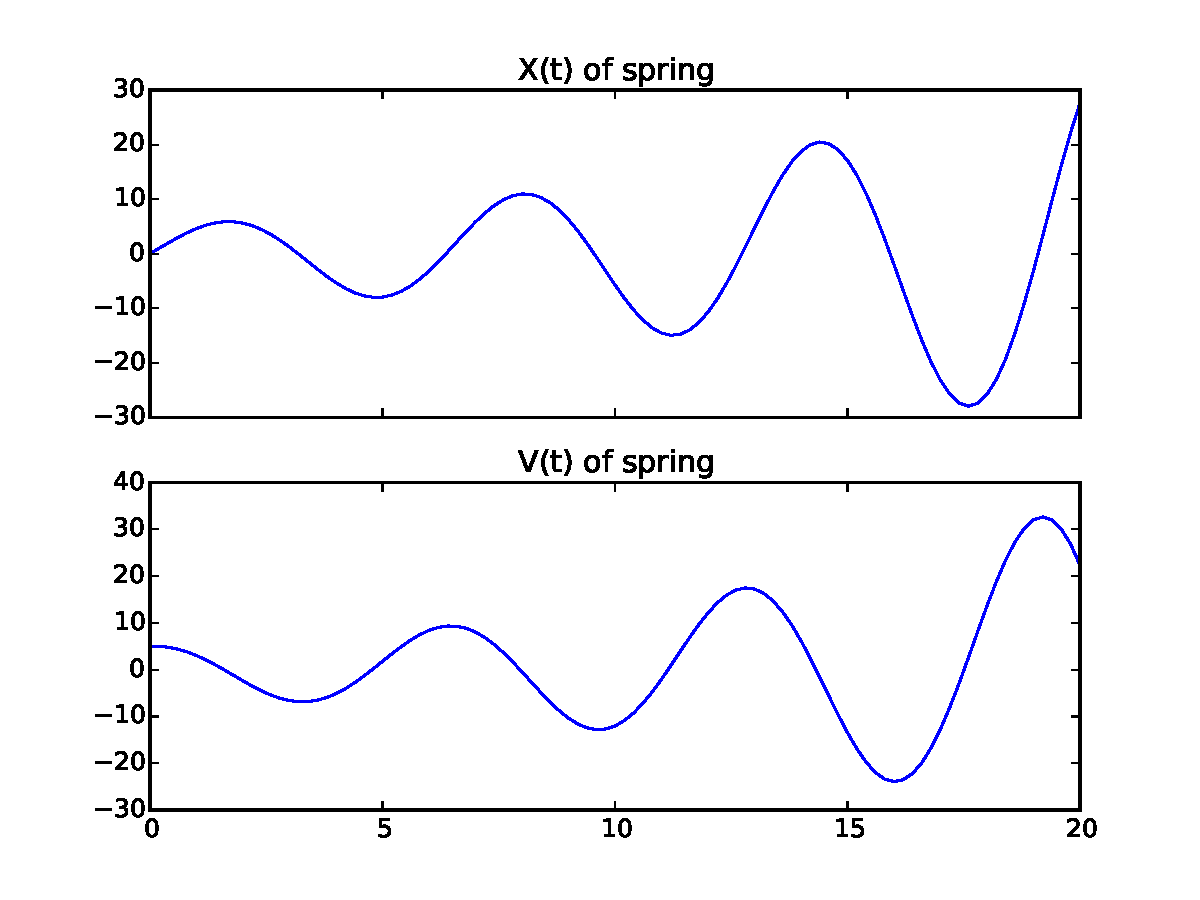
\includegraphics[scale=1.0]{explicitEuler1}
\end{center}


Problem 2. 

I have done this a bunch of times and I'm sure my grader has too, so I'm going to skip a lot of steps.
\begin{equation}
   \textrm{Differential equation: } \quad  m * \ddot{x} + k * x = 0 
\end{equation}
\begin{equation}
   \textrm{We're setting k/m = 1 for convenience. } \quad \ddot{x} + x = 0 
\end{equation}
\begin{equation}
   \textrm{Thus the answer is: } \quad  x(t) = v_{0}*Sin(t) + x_{0}*Cos(t) \quad \textrm{where $v_{0}$ is initial velocity and $x_{0}$ is initial position. }
\end{equation}

\clearpage

\begin{center}
    \textbf{Figure 2: Explicit Euler Errors (same input as Figure 1)}\par\medskip
    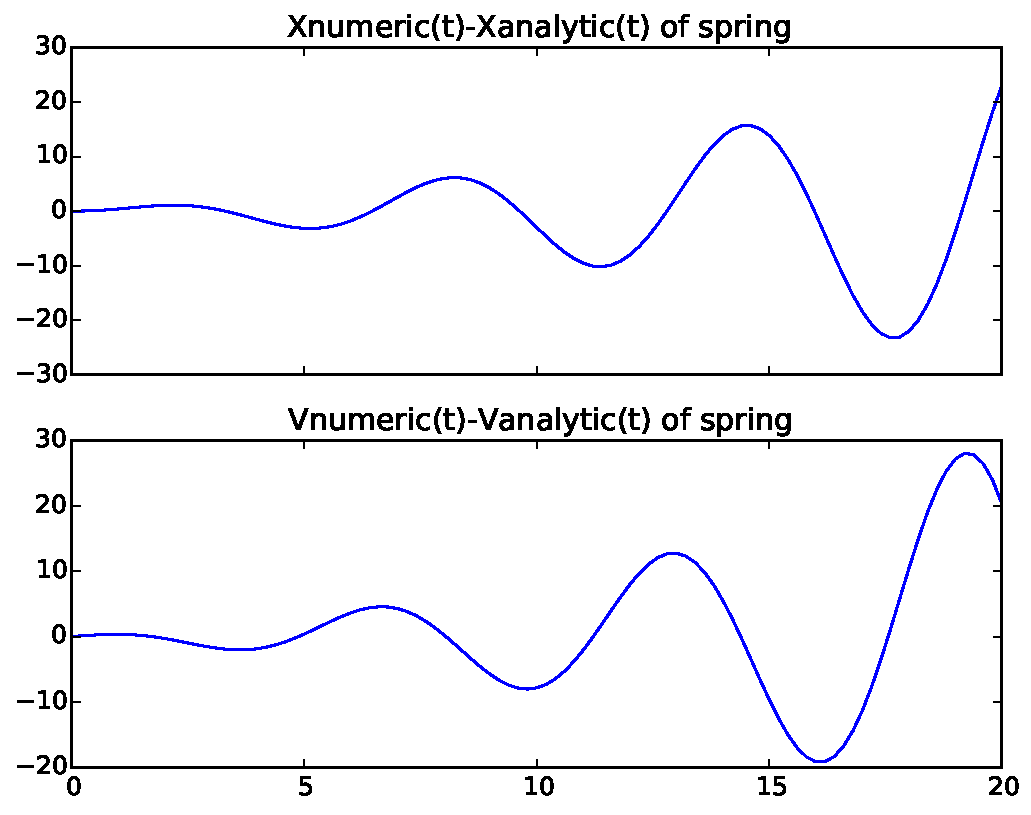
\includegraphics[scale=1.0]{explicitEulerErrors1}
\end{center}


Problem 3.

\begin{center}
    \textbf{Figure 3: Explicit Euler Truncation Errors as a function of h}\par\medskip
    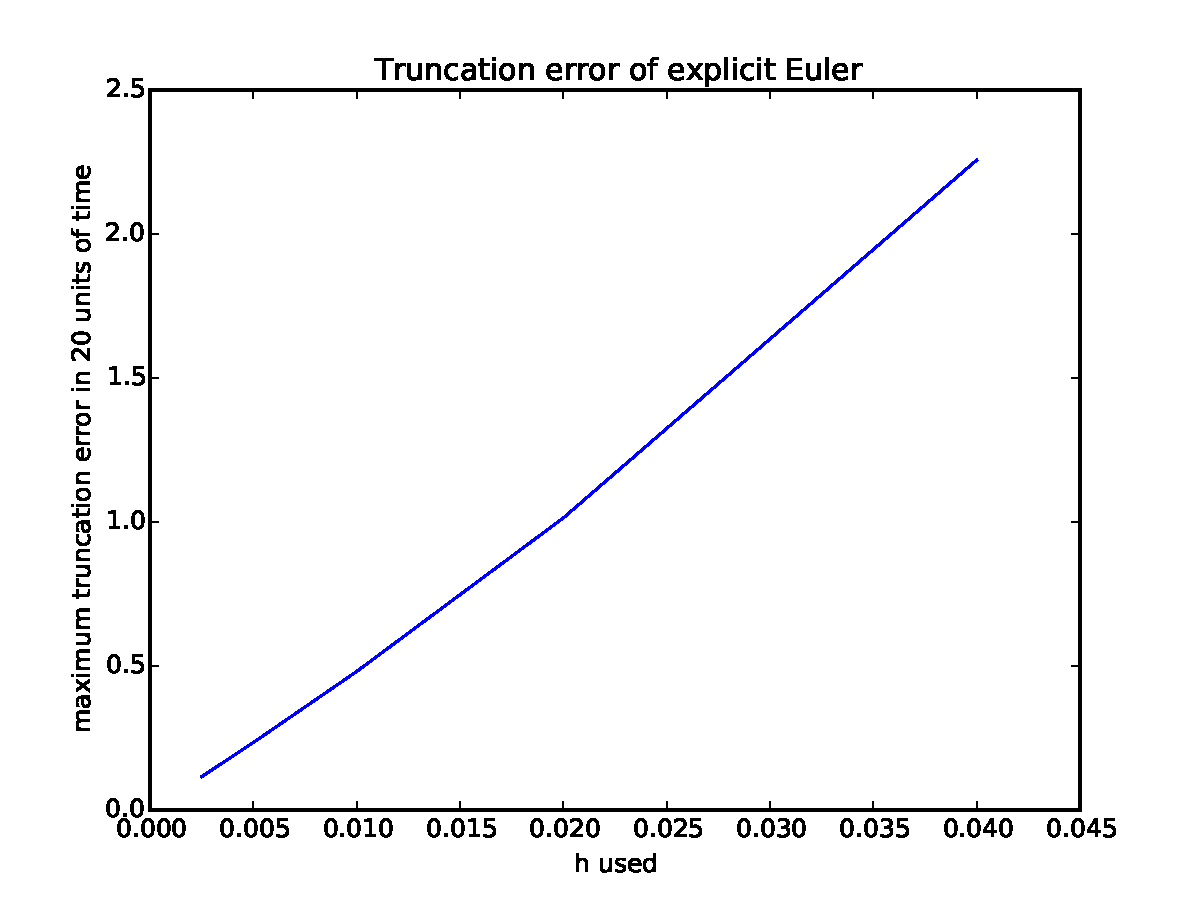
\includegraphics[scale=1.0]{eEtruncation}
\end{center}

Pretty close to linear--and it only gets moreso as h gets smaller.

\bigskip

\clearpage

Problem 4.

\begin{center}
    \textbf{Figure 4: Explicit Euler Energy (same input as Figure 1)}\par\medskip
    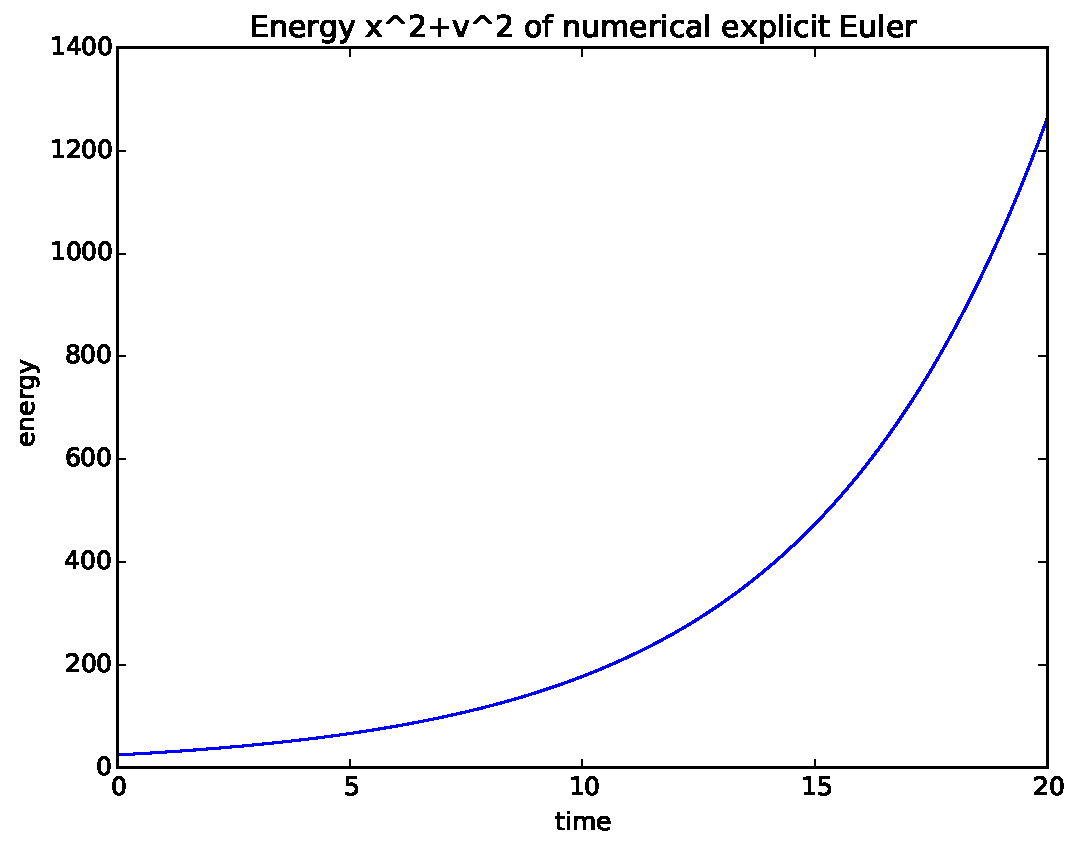
\includegraphics[scale=1.0]{eE_energy}
\end{center}

Just like the errors in x and v, it starts fairly linear in time but quickly becomes exponentially worse.


\bigskip

Problem 5.

We're starting from the implicit Euler methods:

\begin{equation}
    x_{i+1} = x_{i} + h*v_{i+1}  \qquad   v_{i+1} = v_{i} - h*x_{i}
\end{equation}
Now we simply solve a linear system of two equations in two unknowns.
\begin{equation}
    v_{i+1} = v_{i} - h*(x_{i} + h*v_{i+1})
\end{equation}
\begin{equation}
    v_{i+1} = \frac{v_{i} - h*x_{i}}{1 + h^2}
\end{equation}
\begin{equation}
    x_{i+1} = x_{i} + h*(\frac{v_{i} - h*x_{i}}{1 + h^2})
\end{equation}
\begin{equation}
    x_{i+1} = \frac{x_{i} + h*v_{i}}{1 + h^2}
\end{equation}

And now the results:

\begin{minipage}{1.0\textwidth}
\begin{center}
    \textbf{Figure 5: Implicit Euler (same input as Figure 1)}\par\medskip
    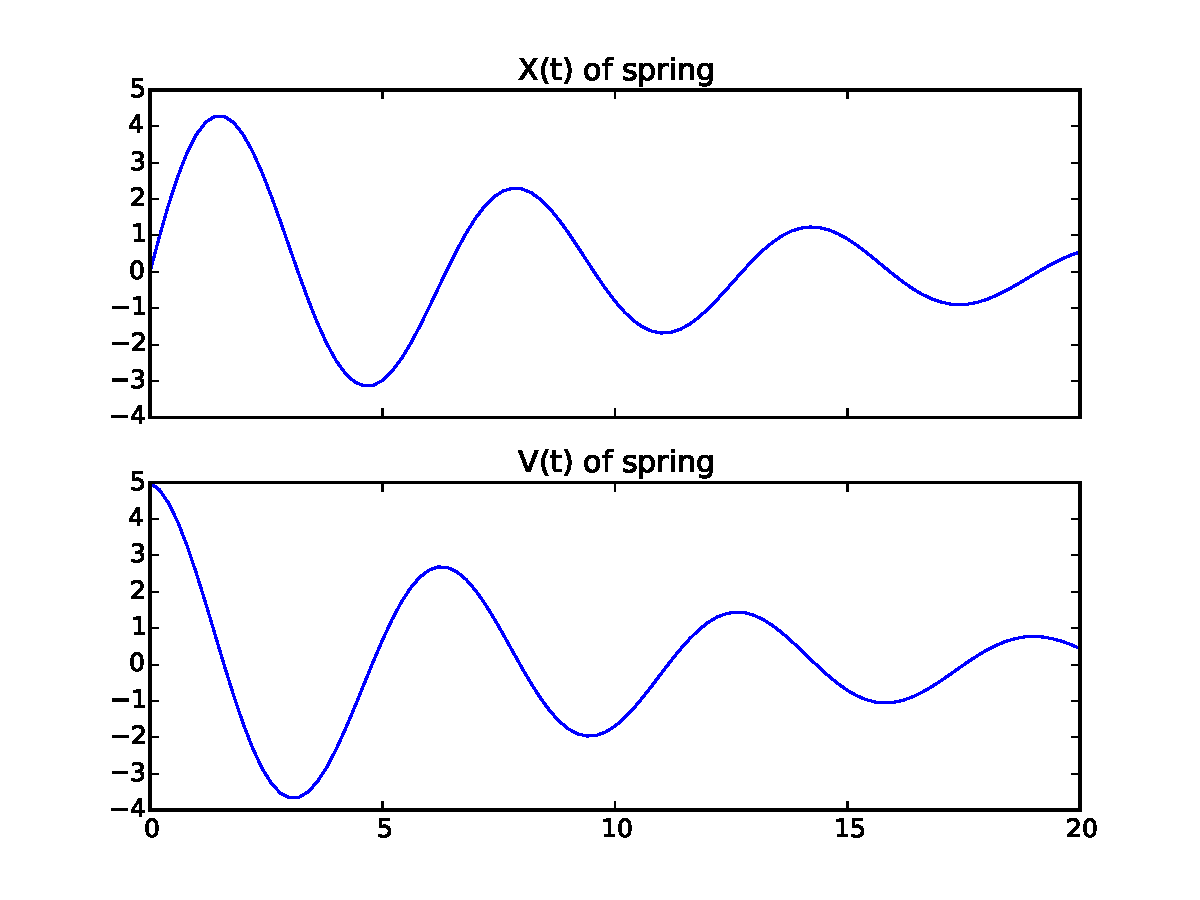
\includegraphics[scale=1.0]{implicitEuler1}
\end{center}
\end{minipage}

Compare to the analytic solution:

\begin{minipage}{1.0\textwidth}
\begin{center}
    \textbf{Figure 6: Implicit Euler Errors (same input as Figure 1)}\par\medskip
    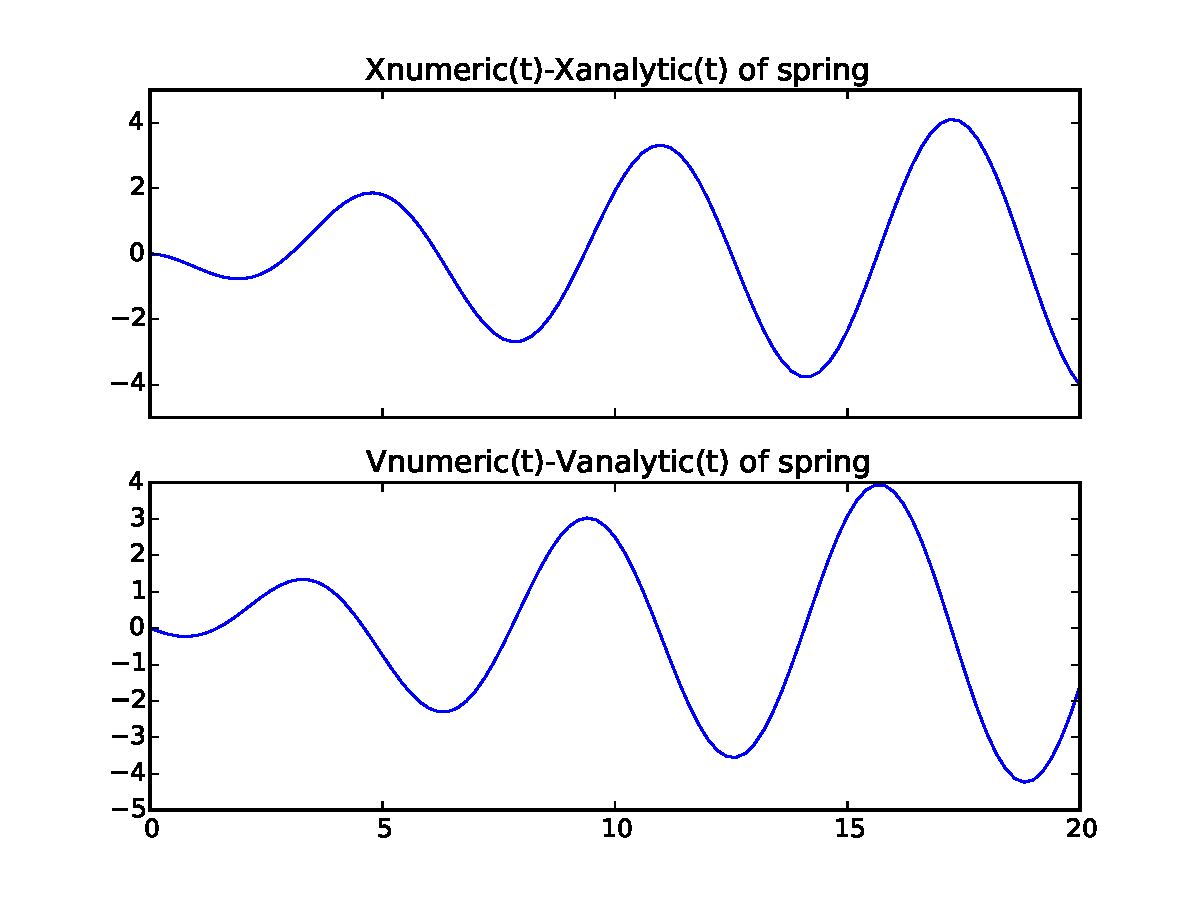
\includegraphics[scale=1.0]{implicitEulerErrors1}
\end{center}
\end{minipage}

We see here that Implicit Euler has the opposite effect of explicit Euler; explicit Euler ``creates'' energy, while implicit euler ``destroys'' energy, at roughly the same rate. Let's check this with the energy.

\begin{minipage}{1.0\textwidth}
\begin{center}
    \textbf{Figure 7: Implicit Euler Energy (same input as Figure 1)}\par\medskip
    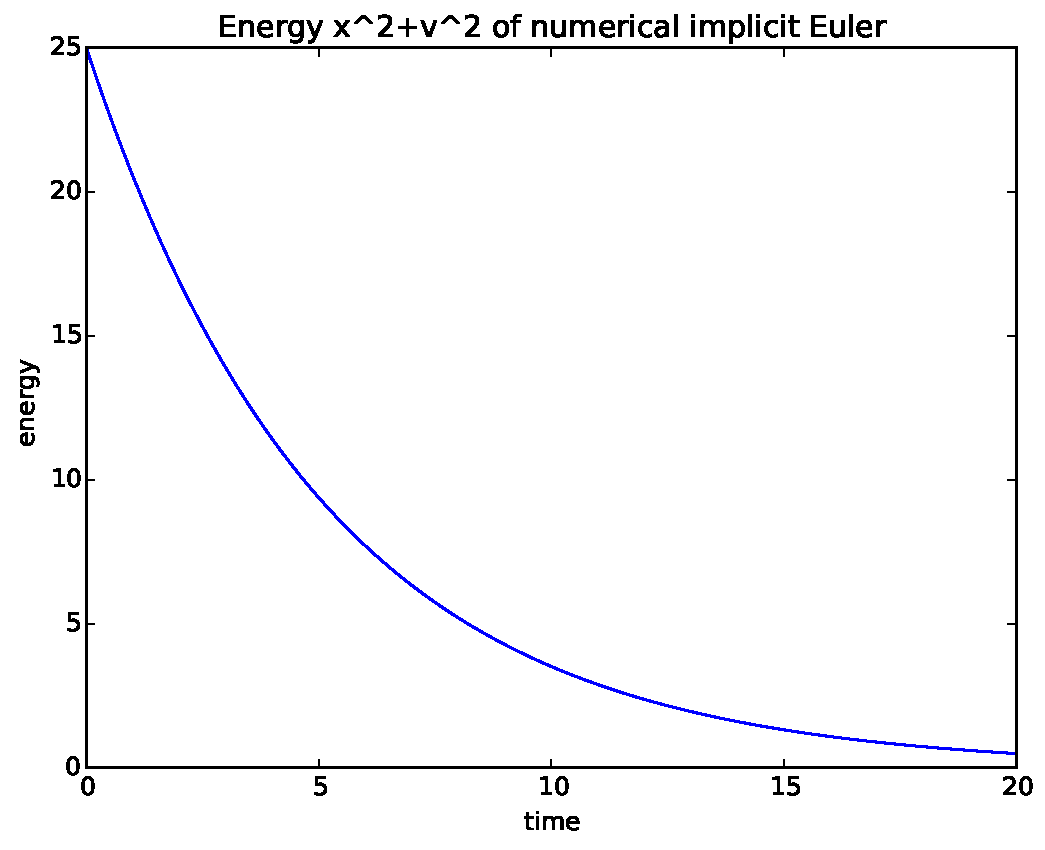
\includegraphics[scale=1.0]{iE_energy}
\end{center}
\end{minipage}

This confirms our expectation; the decrease in energy is roughly linear at the start but quickly becomes exponential.


\clearpage
Rita Sonka

Ph 20

homework set 3 PART 2

10/11/2016

\bigskip

Problem 1.

\begin{minipage}{1.0\textwidth}
\begin{center}
    \textbf{Figure 8: Explicit and Implicit Euler in Phase Space (same input as Figure 1)}\par\medskip
    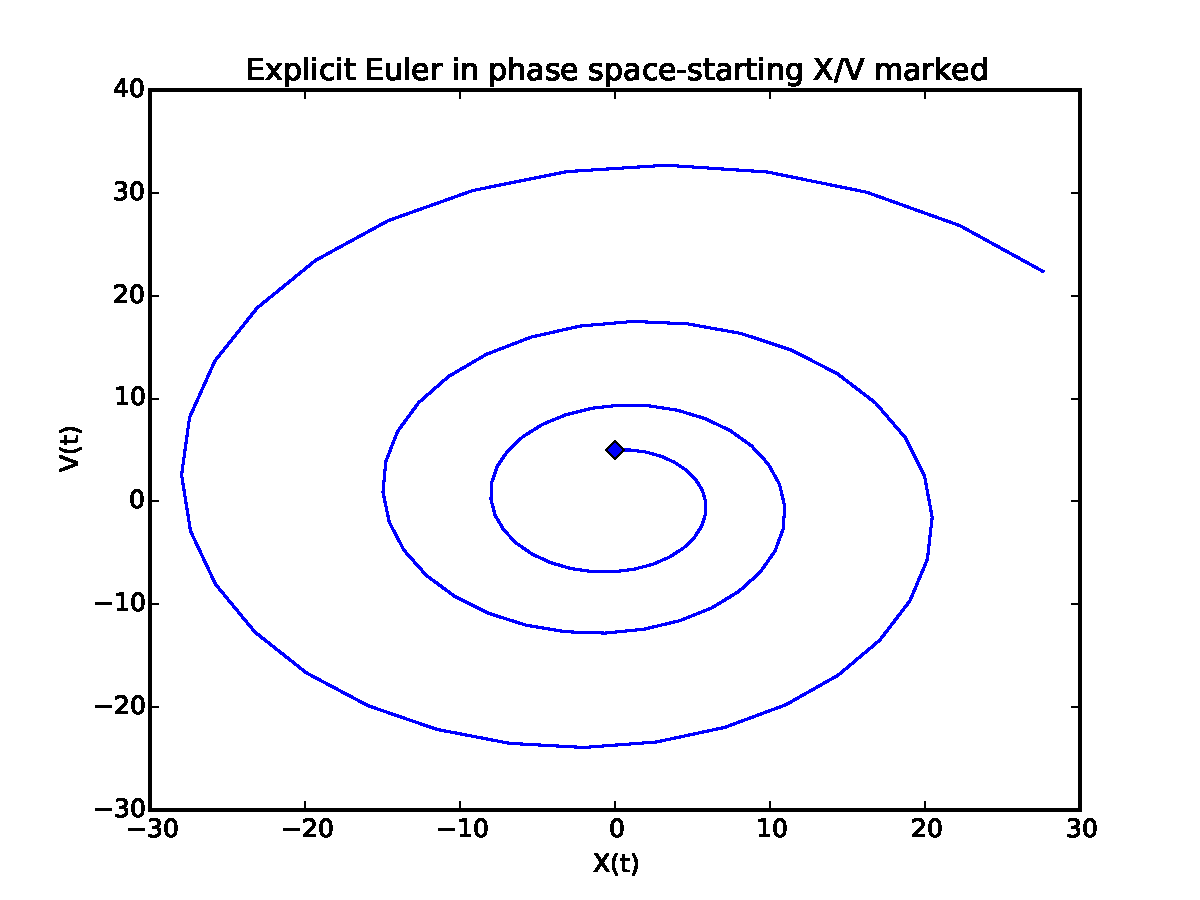
\includegraphics[scale=0.7]{eE_phaseSpace}
    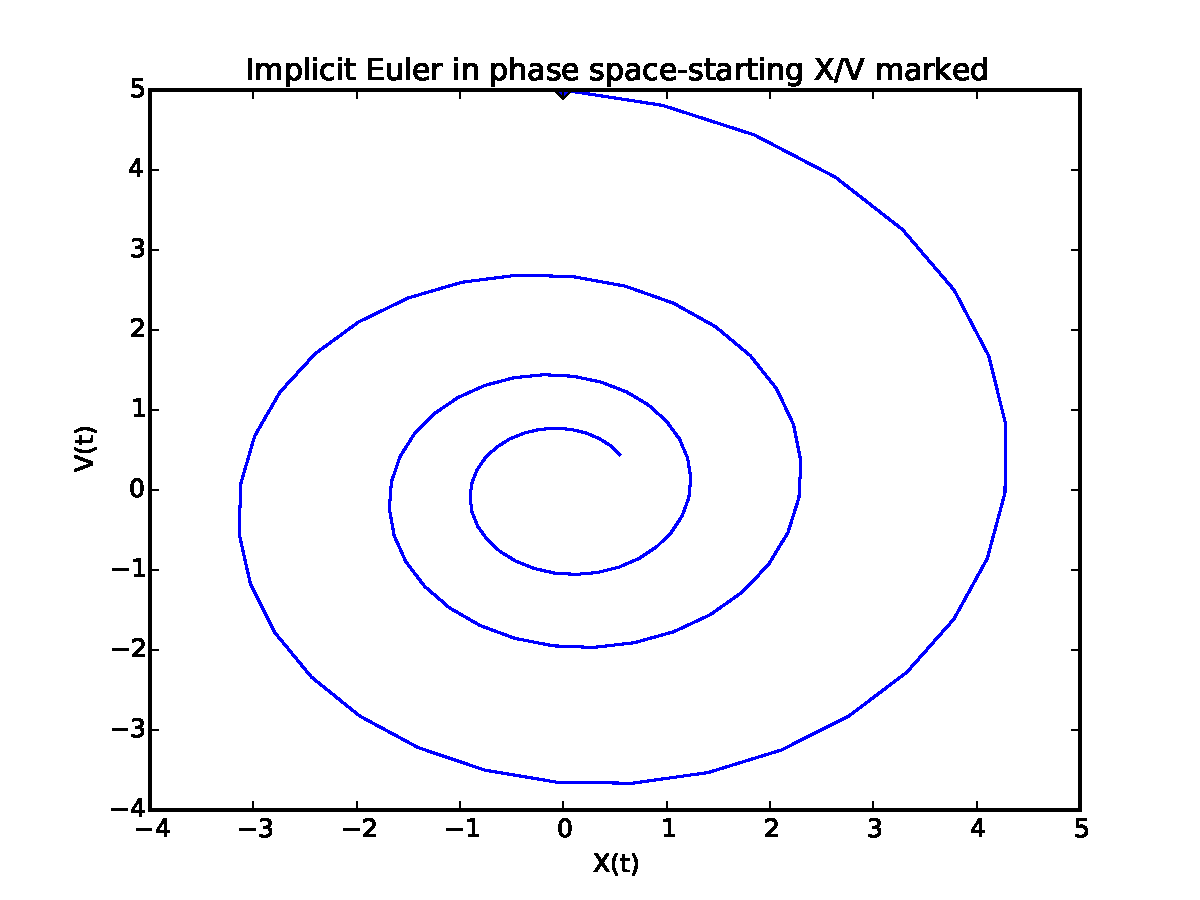
\includegraphics[scale=0.7]{iE_phaseSpace}
\end{center}
\end{minipage}

This pretty clearly demonstrates what we had already found--the explicit Euler increases in energy with time, while Implicit Euler decreases in energy with time. In phase space, this corresponds to Explicit Euler spiraling outwards and Implicit Euler spiralling inwards.

\bigskip

Problem 2.


\begin{minipage}{1.0\textwidth}
\begin{center}
    \textbf{Figure 9: Symplectic Euler in Phase Space (same input as Figure 1)}\par\medskip
    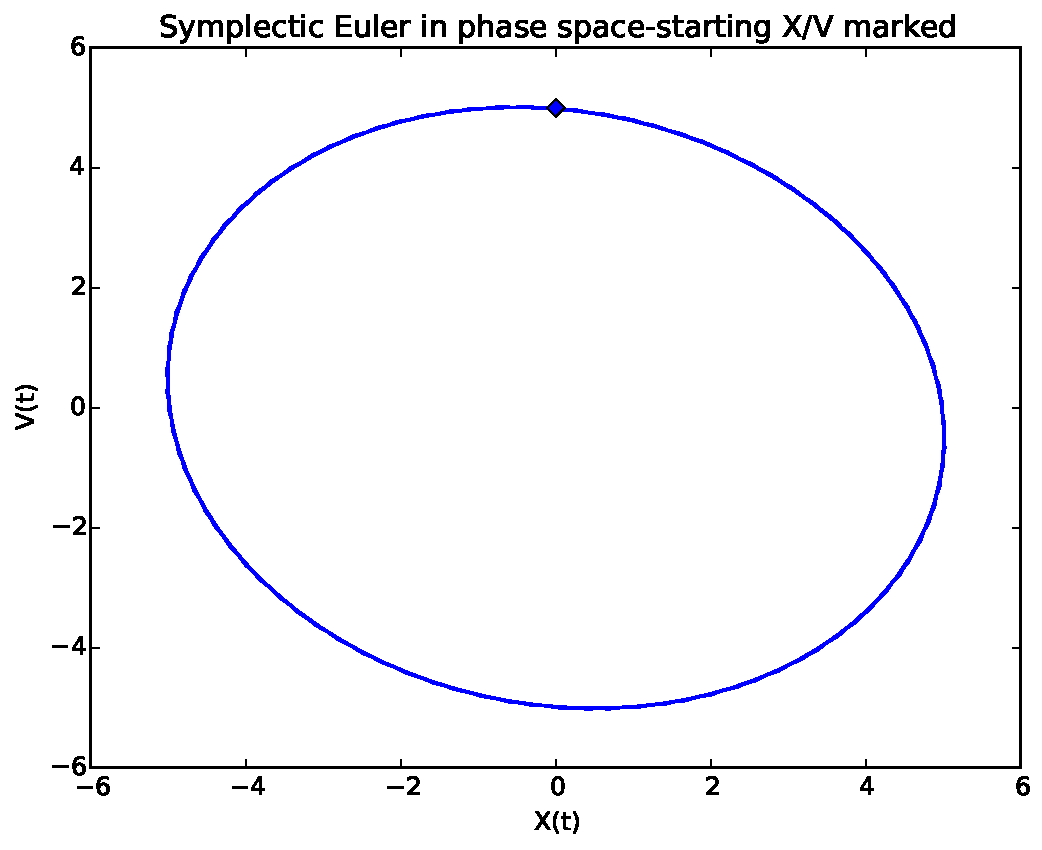
\includegraphics[scale=0.7]{symp_phaseSpace}
\end{center}
\end{minipage}

Unlike Explicit or Implicit Euler, Symplectic Euler DOES conserve energy (on the average, anyway)--we see that it makes a (seemingly) closed circuit of the origin. However, this closed circuit is not a circle--for any time t, the exact values of X and V will likely be off (hard to tell exactly just from phase space). 

\bigskip

Problem 3.

\begin{minipage}{1.0\textwidth}
\begin{center}
    \textbf{Figure 10: Symplectic Euler Energy (same input as Figure 1)}\par\medskip
    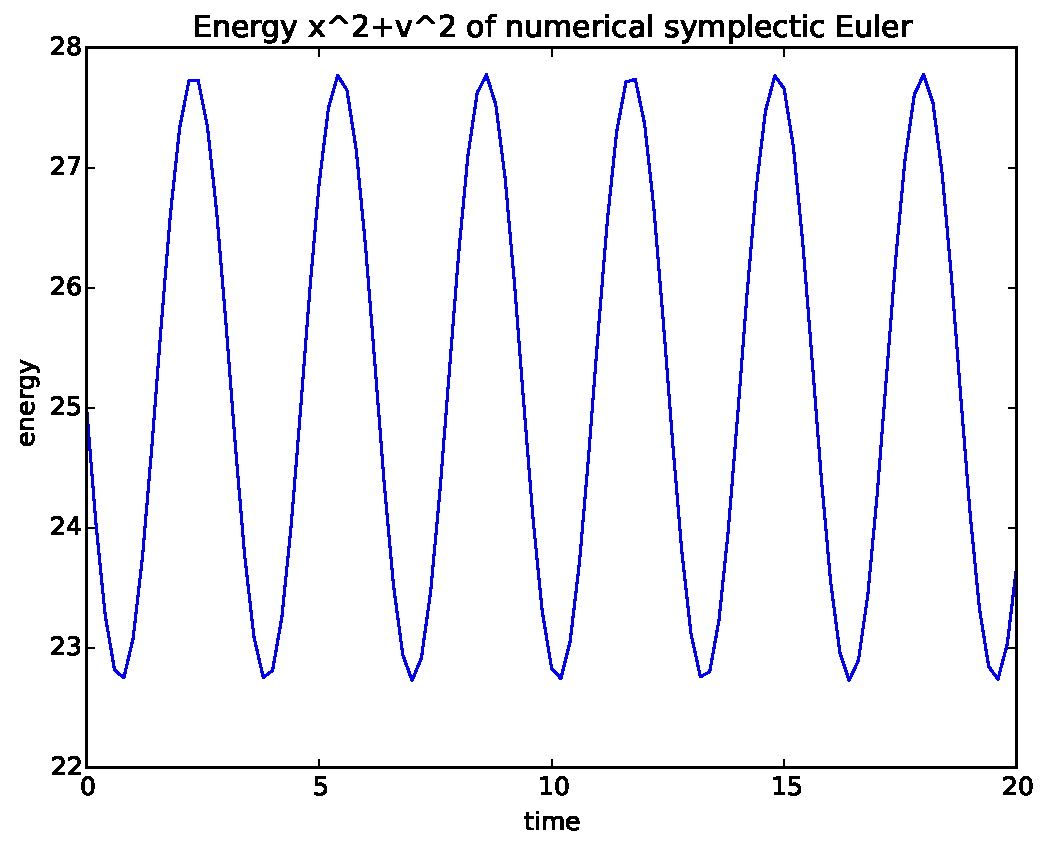
\includegraphics[scale=1.0]{symp_energy}
\end{center}
\end{minipage}

This gives a greater idea of the time evolution of the error. We see a sinusoidal variation in $v^2 + x^2$ with time, corresponding to the ellipse we saw in phase space. So over time it will on average have the right energy, but at any one point the x or v or both is/are likely off.

\bigskip

Problem 4.

\bigskip

\begin{minipage}{1.0\textwidth}
\begin{center}
    \textbf{Figure 11: Symplectic Euler phase difference (same input as Figure 1, except N = 750-1000 instead of 0-100)}\par\medskip
    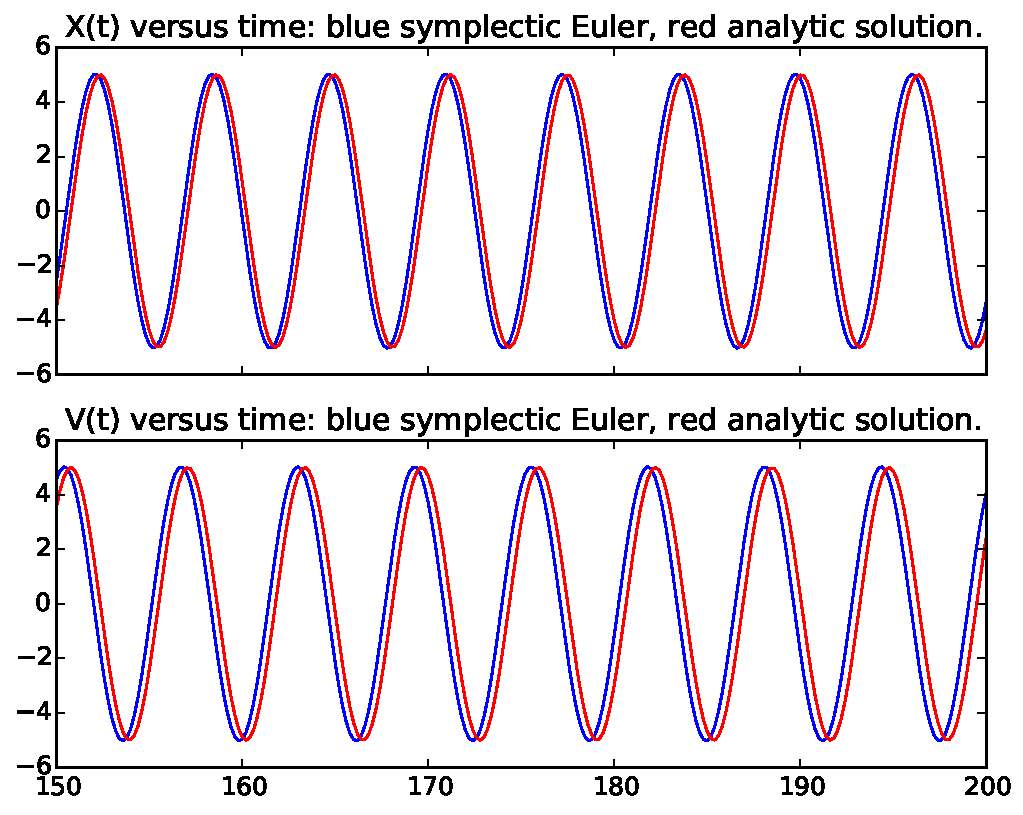
\includegraphics[scale=1.0]{symp_lag}
\end{center}
\end{minipage}

While it isn't obvious from this graph, the v(t) has actually been off by that exact amount since the very beginning, and has neither grown nor shrank. The X(t) on the other hand is clearly getting out of phase over the long term. So I guess that phase diagram would slowly turn into a very fuzzy ellipsoid if I had taken it out long enough.


\end{document}















\begin{comment}
===============================================================================
USEFUL THINGS I'VE DONE BEFORE.


images.
\begin{minipage}{1.0\textwidth}
\begin{center}
    \textbf{Figure 1: Difference in convergence}\par\medskip
    \includegraphics[scale=0.7]{relativeRate}
\end{center}
\end{minipage}

Inline equations
Divide the interval to be integrated [a, b] into N equally-spaced partitions of size $h_{N} = (b-a)/N$; label the partitioning points $x_{0}, x_{1}, ... x_{N}$, with $x_{0} = a, x_{N} = b$. 


non-inline equations.
\begin{equation}
   \frac{4}{6}( f(a)H + f'(a)(\frac{H}{2})^2 + \frac{f''(a)}{2!}(\frac{H}{2})^3 + \frac{f'''(a)}{3!}(\frac{H}{2})^4 + \frac{f^{(4)}(\eta)}{4!}(\frac{H}{2})^5 ) +
\end{equation}
\begin{equation}
   \frac{1}{6}( f(a)H + f'(a)H^2 + \frac{f''(a)}{2!}H^3 + \frac{f'''(a)}{3!}H^4 + \frac{f^{(4)}(\eta)}{4!}H^5 ) \qquad \mathrm{ Hi this is normal text.} \quad \textrm{This is too.} \: 
\end{equation}

formatting:
\clearpage
\bigskip

\end{comment}
